

\chapter{The martingale approach to option pricing}\label{Chapter2}
%\blindtext
\minitoc% Creating an actual minitoc

\vspace{5em}


In mathematical finance, one of the key issues is to find the fair price of a financial derivative. 
A financial derivative is a security whose value depends on the price of one or more basic securities 
such as stocks or bonds (the so called \textbf{underlying assets}). 
A \textbf{European call} option on a security with price process $\{S_t\}_{t\geq0}$, is the right to
buy the security at the predetermined exercise price $K$ (also called \textbf{strike}). This right may be exercised at the expiration date $T$ (also called \textbf{maturity}) 
of the option.
The call option can be purchased at the price $C_{t_0}$ at time $t_0=0<T$.
A \textbf{European put} option is similar, but gives the owner the right to sell the underlying asset at the strike price at maturity. 
In contrast to European options, \textbf{American options} can be exercised at any time between the writing and the expiration of the contract.
The value of the option at the exercise time $\tau$ such that $0 \leq \tau \leq T$, is called \textbf{payoff}, and has the form
$$ \mbox{Call:} \quad C_{\tau} = \max \{ S_{\tau} - K, 0 \} $$
$$ \mbox{Put:} \quad P_{\tau} = \max \{ K - S_{\tau}, 0 \} $$
Because of the $\max$ operator in the payoff, the options are nonlinear instruments. 

Determining the correct price of an option is not a simple task. 
It requires a stochastic model for the dynamics of the underlying price and several assumptions on the market.
The solution of this problem has been presented for the first time in the celebrated paper \cite{BS73}. 
The standard Black-Scholes (BS) model is built on the concept of \textbf{ideal market}, where all the following 
conditions are fulfilled:
\begin{enumerate}
 \item \emph{There are no arbitrage possibilities} (see Definition \ref{arbitrage_def}).
 \item \emph{Exists a risk free asset $B$ with dynamics
        \begin{equation}
         dB_t = r_t B_t dt
        \end{equation}
        where $r_t$ is the deterministic risk free interest rate.}
 \item \emph{It is possible to borrow and lend any amount of cash, even fractional, at the risk free rate.}
 \item \emph{It is possible to buy and sell any amount, even fractional, of the stock. This includes short selling.}
 \item \emph{The market is frictionless.}
 \item \emph{For $\mu \in \R$ and $\sigma > 0$, the underlying stock process $\{S_t\}_{t\geq 0}$ follows the geometric Brownian motion}
	\begin{equation}\label{GBM2}
	  \frac{dS_t}{S_t} = \mu dt + \sigma dW_t.
	\end{equation}
\item \emph{The stock does not pay dividends.}	
\end{enumerate}

This is a modern formulation, taken from \cite{Musiela}, of the original assumptions presented in the article \cite{BS73}.
By relaxing one or more of the previous hypothesis, it is possible to develop new models that usually are generalizations of the standard BS model. 
For instance, it is common to relax the hypothesis (7) in order to extend the model to stocks that pay dividends. In this thesis we will not do it.

The hypothesis of \emph{frictionless market} implies that the cost of trading is zero. This means that: all investors are price takers (no market impact), 
all parties have the same access to the relevant information, there are no transaction costs or commissions, and all assets are
assumed to be perfectly divisible and liquid.
Transaction costs can be divided in two categories: costs that are proportional to the price of the traded security, and fixed costs. 

In this thesis we relax the hypothesis (5) by introducing proportional transaction costs, and the hypothesis (6) by replacing the geometric Brownian motion
with an exponential Lévy process.

In this chapter, we present the basic concepts of the ``No-arbitrage'' pricing theory and the numerical algorithms based on the finite difference method. 
We will see that the pricing model can always be represented by a partial integro-differential equation 
(PIDE) when the stock dynamics follows an exponential Lévy process. 


\section{No arbitrage theory}\label{No_arbitrage_theory}

All the mathematical framework for derivative pricing is based on the concept of \textbf{No-Arbitrage}.\\
It is convenient to introduce some useful definitions.
\begin{Definition}
 Let us consider a financial market containing a stock with price process $\{S_t\}_{t\geq0}$ defined on the probability space 
 $(\Omega,\mathcal{F},\{\mathcal{F}_{t}\}_{t\geq0},\PP)$. \\
 A \textbf{financial derivative} (or contingent claim)\footnote{ 
 With the term ``contingent claim" some authors indicate only contracts with an optionality. In this thesis we follow the nomenclature of \cite{Bjork} and \cite{Musiela}.} 
 with maturity $T$
 is any $\mathcal{F}_{T}$-measurable random variable $\mathcal{X}$.
 
 A financial derivative is called ``simple" if it is of the form $\mathcal{X} = \Phi(S_{T})$. The function $\Phi$ is called the \textbf{payoff}.  
\end{Definition}
We see that European call and put options are simple financial derivatives. 
All European path dependent options are examples of non-simple derivatives. In thesis we will consider only simple derivatives. 
Also American-style contracts are included into this definition if we replace 
the maturity date $T$ with the exercise date $\tau$ such that $\tau \leq T$. 
However, in this chapter we do not consider such instruments because their pricing formula requires the introduction of a more complex framework i.e.
optimal stopping theory.

\begin{Definition}
 Let us consider a stock with (cádlág) price process $\{S_t\}_{t\geq0}$ and a risk free asset with process $\{B_t\}_{t\geq0}$.
 \begin{enumerate}
  \item A \textbf{portfolio} is a pair of predictable processes $(\alpha_t, \beta_t)_{t\geq0}$ describing the amount of each asset held by the investor. 
  \item The value of such a portfolio at time $t$ is
  $$ \varTheta_t = \alpha_t S_t + \beta_t B_t. $$
  The process $\{\varTheta_t\}_{t\geq0}$ is called \textbf{portfolio value process}.
  \item A portfolio $(\alpha_t, \beta_t)_{t\geq0}$ is said to be \textbf{self-financing} if 
  \begin{equation}\label{self_financing}
     \varTheta_t = \varTheta_0 + \int_{0^+}^t \alpha_u dS_u + \int_{0^+}^t \beta_u dB_u. 
  \end{equation}
\end{enumerate}
\end{Definition}
The meaning of equation (\ref{self_financing}) is that the value of the portfolio at time $t$ is equal to the initial value $\varTheta_0$ plus
the capital gain between $0$ and $t$.

\begin{Definition}\label{arbitrage_def}
 An \textbf{arbitrage} is a self-financing portfolio value process $\{\varTheta_t\}_{t\geq0}$ satisfying $\varTheta_0=0$ and also for some $T>0$
 $$ \PP\bigl( \varTheta_T \geq 0 \bigr) = 1 \quad \mbox{and} \quad \PP\bigl( \varTheta_T > 0 \bigr) > 0. $$
\end{Definition}
An arbitrage is a trading strategy such that an investor starts with zero capital and at some later time $T$ he is sure to have lost no money and furthermore has a positive
probability of having made a profit.

We can define the discount factor for $0 \leq s \leq t \leq T$ as
\begin{equation}\label{discount_factor}
 D(s,t) = e^{-\int_s^t r_u du}.
\end{equation}
In the following of this thesis we assume a constant interest rate $r_u = r$ for all $u \in [0,T]$. \\
It is common to indicate with $\PP$ the physical probability measure and with $\Q$ a risk neutral measure, also called equivalent martingale measure (EMM).
\begin{Definition}
 Given the asset price process $\{S_t\}_{t\geq0}$ defined on the probability space 
 $(\Omega,\mathcal{F},\{\mathcal{F}_{t}\}_{t\geq0},\PP)$, we say that the probability measure $\Q$ is an \textbf{EMM}
 if it verifies the following two properties:
 \begin{equation}
 \Q \sim \PP : \quad \forall A \in \mathcal{F} \quad \quad \Q(A) = 0 \Leftrightarrow \PP(A) = 0,  
 \end{equation}
\begin{equation}
 D(0,t) S_t = \E^{\Q} \bigl[ D(0,T) S_T \big| \F_t \bigr] \quad \mbox{for} \quad 0\leq t \leq T.
\end{equation}
\end{Definition}

Our main problem is to determine the
fair price $\Pi_t(\mathcal{X})$ of the derivative $\mathcal{X}$ at time $t$ (with $0 \leq t \leq T$).
There are some minimal requirements that $\Pi_t(\mathcal{X})$ should verify to qualify as a pricing rule:
\begin{enumerate}
 \item It should be possible to price a derivative using only the information given at time $t$.
 \item A derivative with a positive payoff should have a positive value.
 \item Linearity.
\end{enumerate}
In \cite{Cont} (see Proposition 9.1), the authors prove that any arbitrage-free linear pricing rule $\Pi_t(\mathcal{X})$ satisfying the properties above, 
is represented by the \emph{risk neutral} pricing rule
\begin{equation}\label{derivative_price}
 D(0,t) \Pi_t(\mathcal{X}) = \E^{\Q} \bigl[ D(0,T) \mathcal{X} \big| \F_t \bigr] \quad \mbox{for} \quad 0\leq t \leq T,
\end{equation}
where $\Q$ is an EEM.

The concept of arbitrage is related with the existence of an equivalent martingale measure through the \textbf{first fundamental theorem of asset pricing}.
\begin{Theorem}
 A market model does not admit arbitrage if and only if there exists a risk-neutral probability measure. 
\end{Theorem}
For a detailed proof we refer to the academic literature on this topic i.e. \cite{HaKr79}, \cite{HaPl81}, \cite{Sch02}, \cite{DelSch98}.
The general No-arbitrage theory of asset pricing is a fundamental and sophisticated theory of mathematical finance with several important developments 
in the last forty years, and we do not discuss it in details in this thesis.
For a general presentation of this theory we refer to \cite{Bjork} (Chapter 10.2). For a comprehensive introduction, 
considering discontinuous processes, we refer to \cite{Cont} (Chapter 9.1).

Another important concept originating in the Black-Scholes model is the concept of perfect hedge.
\begin{Definition}
 A self-financing portfolio $(\alpha_t,\beta_t)$ is said to be a \textbf{perfect hedge} (or \textbf{replicating portfolio}) for a derivative  
 $\mathcal{X}$ if the associated portfolio value process $\{\varTheta_t\}_{t\geq0}$ satisfies
 \begin{equation}\label{perfect-hedge}
    \mathcal{X}  = \varTheta_T   \quad \quad \PP \mbox{ - almost surely}. 
  \end{equation}
\end{Definition}
If the market is arbitrage-free and
(\ref{perfect-hedge}) holds under $\PP$, it must hold also under $\Q$, since they are equivalent.

The initial value $\varTheta_0$ is the price of the derivative at time $0$.
Using (\ref{perfect-hedge}) and (\ref{self_financing}), under $\Q$ we can write  
$D(0,T) \mathcal{X} = \varTheta_0 + \int_{0+}^T \alpha_t \, d\bigr( D(0,t)S_t \bigr)$. Since the discounted price $D(0,t)S_t$ under $\Q$ is a martingale, the stochastic integral  
$\int_{0+}^T \alpha_t \, d\bigr( D(0,t)S_t \bigr)$ is a martingale as well. By taking the expectation we obtain:
\begin{equation}
   \Pi_0(\mathcal{X}) = \E^{\Q} \bigl[ D(0,T) \mathcal{X} \big| \F_t \bigr] = \varTheta_0.
\end{equation}
Moreover, the initial value $\varTheta_0$ is unique, since two replicating strategies with different initial values lead to an arbitrage.
\begin{Definition}
 A market model is said to be \textbf{complete} if the payoff of every derivative security can be perfectly hedged. 
\end{Definition}
In a complete market, the unique price of a financial derivative corresponds to the initial capital $\varTheta_0$ needed to set up a perfect hedge.

The completeness of a market is connected with the uniqueness of the EMM through the
\textbf{second fundamental theorem of asset pricing}.
\begin{Theorem}
 Consider a market model that has a risk-neutral probability measure. The model is complete if and only if the risk-neutral probability measure is unique.
\end{Theorem}
The theorem as stated above holds in discrete time models. In continuous time this formulation is not rigorous. 
It is necessary to carefully define the set of admissible trading strategies, contingent claims and the
notion of martingale measure. 
In the case where the stock process has unbounded jumps, which is the case of most exponential Lévy models, a rigorous formulation is quite difficult
and we refer to \cite{ChSh02} and \cite{Kabanov01} for more information.

The ideal market assumed by Black and Scholes is complete (see Theorem 8.3 of \cite{Bjork}). 
However, the majority of the models used in finance are not.

In this thesis we analyze a market model that is not complete. The introduction of proportional transaction costs prevents to trade continuously in time  
as suggested by the replicating portfolio strategy, because the cost of trading would be infinity.
On the other hand, if we consider exponential Lévy models, we again obtain an incomplete market in general,
except for some particular cases i.e. when the driving noise is a Brownian motion or a pure Poisson process.
%The reason is that the unpredictable jumps of a Lévy process are a source of risk that cannot be hedged by the replicating strategy.

In a complete market there is only one arbitrage-free way to price a financial derivative, and the price is defined as the cost to replicate the derivative's payoff.
In an incomplete market, instead, the notion of perfect replication does not exist. 
Therefore the hedging strategy will only approximate the payoff of the derivative. Different ways to measure the risk of trading lead to different 
ways to hedge the derivative. In this thesis we focus on the approach based on the concept of \emph{utility maximization} (see Chapter \ref{Chapter5}).

In the following of this chapter we consider a frictionless market where the stock price follows an exponential Lévy process. 
In in such a market, the class of EMM is infinite, 
i.e. there are infinite EMMs such that the discounted stock prices are martingales.
This means that for every financial derivative there are infinite prices satisfying the condition of no-arbitrage. 

In order to overcome this problem, there are several methods to select the best EMM to use in the pricing formula (\ref{derivative_price}) (
see \cite{Cont}, Chapter 10).
However, the best approach is to derive the model parameters directly from the prices of derivatives (usually European call and put options with different strikes and maturities) 
already quoted in the market.
The process of choosing the risk neutral parameters for a model, such that it reproduces the prices in the market is called \emph{model calibration}.
In this chapter all the parameters of the Lévy processes used for the pricing purpose, are intended to be risk neutral parameters obtained by a calibration process.





\subsection{Derivation of the price PIDE}

In an arbitrage-free market, if the price process $\{S_t\}_{t\geq0}$ follows an exponential Lévy process, 
we can express the price of any simple financial derivative $\mathcal{X}$ as a function of the current time 
$t \in [0,T]$ and current stock price $s=S_t$, i.e. $\Pi_t(\mathcal{X}) = V(t,s)$.
This is a direct consequence of the Markov property (\ref{Markov_prop}) applied to the formula (\ref{derivative_price}).
In this section we show that $V(t,s)$ can be obtained by solving a partial integro-differential equation (PIDE).

First of all, let us define the space of continuous functions that have polynomial growth of order $p$ at infinity.
\begin{Definition}\label{Cp}
 For $E \subseteq \R^n$ and for $p\geq 0$, let us define the space:
\begin{equation}
 \mathcal{C}_p \bigl( E \bigr) = \left\{  \phi \in C^0\bigl( E \bigr) : \sup_{E} 
 \frac{|\phi(x)|}{1+|x|^p} <\infty   \right\}. 
\end{equation}
\end{Definition}
For functions with time dependence, e.g. $\phi : [0,T] \times \R^n \to \R$, we maintain the same notation but specify the domain: 
\begin{equation}
 \mathcal{C}_p \bigl([0,T] \times \R^n \bigr) = \left\{  \phi \in C^0\bigl( [0,T] \times \R^n \bigr) : \sup_{[0,T] \times \R^n} 
 \frac{|\phi(t,x)|}{1+|x|^p} <\infty   \right\}. 
\end{equation}
We consider only the case $p=2$, because we are working with underlying processes with finite second moment. (see assumption \textbf{EM} in Section \ref{AssumptionEM} ).

The following theorem will be useful.
\begin{Theorem}
 Let $\{X_t\}_{t\geq0}$ be a Lévy process with Lévy triplet $(b,\sigma,\nu)$, satisfying the assumption EM. 
 The process $\{S_t\}_{t\geq0}$ defined by $S_t = e^{X_t}$ is a martingale if and only if
 \begin{equation}\label{martingale_b}
  b +\frac{1}{2} \sigma^2  + \int_{\R} \bigl( e^z-1 -z\mathbbm{1}_{\{ |z|<1 \}} \bigr) \nu(dz) = 0.
 \end{equation}
\end{Theorem}
\begin{proof}
 The SDE for the process $\{e^{X_t}\}_{t\geq0}$ has been derived in Eq. (\ref{exp_sde}). The exponential Lévy process is a martingale if and only if the drift is zero.
\end{proof}
Let us consider a stock price process described by the \emph{exponential Lévy model}
\begin{equation}\label{ELM2}
 S_t = S_0 e^{L_t} = S_0 e^{rt + X_t}
\end{equation}
where $\{X_t\}_{t\geq 0}$ is a Lévy process with Lévy triplet $(b,\sigma,\nu)$. Under a risk neutral measure $\Q$, the process $\{L_t\}_{t\geq 0}$ 
is a Lévy process with triplet $(r+b,\sigma,\nu)$ 
satisfying (\ref{martingale_b}).  
The discounted price is a $\Q$-martingale:
\begin{equation}
 \E^{\Q} \bigl[ e^{-rt} S_t \bigr| S_0 \bigr] =  \E^{\Q} \bigl[ S_0e^{X_t} \bigr| S_0 \bigr] = S_0, 
\end{equation}
such that $\E^{\Q}[ e^{X_t} | X_0=0] = 1 $. 

In Chapter \ref{Chapter1} we derived the infinitesimal generator for an exponential Lévy process in Eq. (\ref{inf_gen_exp_levy}) and the 
parameter $\mu$ in (\ref{mu}).
We can repeat the same computation that led to Eq. (\ref{exp_sde}) for the process $L_t = X_t + rt$ and define the new parameter
\begin{equation}\label{mu2}
 \mu := r + b + \frac{1}{2}\sigma^2 + \int_{\R} ( e^{z} - 1 -z\mathbbm{1}_{|z|<1}) \nu(dz)
\end{equation}
Using the condition (\ref{martingale_b}) we obtain the fundamental relation
\begin{equation}\label{mu=r}
 \mu = r.
\end{equation}
The risk neutral dynamics of (\ref{ELM2}) is described by the SDE:
\begin{equation}\label{RN_sde}
 d S_t = \; r S_{t^-} dt +  \sigma S_{t^-} dW_t \; + \int_{\R} S_{t^-} (e^{z} - 1) \tilde N(dt,dz). 
\end{equation}
For $f \in C^{2}(\R^+) \bigcap \mathcal{C}_2(\R^+)$, the associated infinitesimal generator is:
\begin{align}\label{RN_inf_gen}
 \LL^S f(s) =& \; r s \frac{\partial f(s)}{\partial s}
+ \frac{1}{2} \sigma^2 s^2 \frac{\partial^2  f(s)}{\partial s^2}  \\ \nonumber
&+ \int_{\R} \biggl[ f(se^z) - f(s) - s(e^z-1)\frac{\partial f(s)}{\partial s} \biggr] \nu(dz).
\end{align}

The derivative pricing function $V(t,s)$ with $t \in [0,T]$ and $s\in \R^+$, can be obtain by solving a pricing PIDE according to the following theorem.
\begin{Theorem}\label{Theorem_PIDE}
 Let us consider an arbitrage free market, where the underlying stock price follows the exponential Lévy process (\ref{ELM2}). 
 Let also assume that $V(t,s) \in C^{1,2}([t_0,T] \times \R^+)$ and the derivatives   %\bigcap \mathcal{C}_2([t_0,T] \times \R^+)$,
 $\frac{\partial V}{\partial t}$, $\frac{\partial V}{\partial s}$ %are in $\mathcal{C}_1([t_0,T] \times \R^+)$
 and $\frac{\partial^2 V}{\partial s^2}$ are bounded.
 % The payoff $\Phi(\cdot)$ is such that $\E[\Phi(S_T)]< \infty$. 
 Therefore $V(t,s)$ satisfies the PIDE
\begin{align}\label{derivative_PIDE}
 & \frac{\partial V(t,s)}{\partial t} + \LL^{S} V(t,s) -r V(t,s) = 0 \\
 & V(T,s) = \Phi(s),
\end{align}
where $\LL^S$ is the infinitesimal generator in (\ref{RN_inf_gen}). 
\end{Theorem}
\begin{proof}
 Let us consider the formula 
 (\ref{derivative_price}) together with the Markov property (\ref{Markov_prop}). 
 For any stopping time $\tau$ such that $0 \leq t \leq \tau \leq T$, we can use the law of iterated expectations:
 \begin{align*}
   D(0,t) V(t,s) &= \E^{\Q}  \biggl[ \E^{\Q} \bigl[ D(0,T) V(T,S_T) \big| S_{\tau} \bigr] \bigg| S_t=s \biggr] \\ 
                 &= \E^{\Q} \bigl[ D(0,\tau) V(\tau,S_{\tau}) \big| S_t=s \bigr]. 
 \end{align*}
 We can write $D(0,\tau) V(\tau,S_{\tau}) = D(0,t) V(t,s) + \int_t^{\tau} d\bigl(D(t,u) V(u,S_u)\bigr) du$. 
 Using the It\=o product rule (\ref{Ito_product}) we get:
 \begin{align}\label{proof_Cont_V}
  0 =& \; \E^{\Q} \biggl[ \int_t^{\tau} e^{-r(u-t)} \biggl( \frac{\partial V(u,S_{u^-})}{\partial u} + \LL^{S} V(u,S_{u^-}) -r V(u,S_{u^-}) \biggr) du \bigg| S_t=s \biggr] \\ \label{term1}
     & + \E^{\Q} \biggl[ \int_t^{\tau} e^{-r(u-t)} \frac{\partial V(u,S_{u^-})}{\partial s} \sigma S_{u^-} \; dW_u \; \bigg| S_t=s \biggr] \\ \label{term2}
     & + \E^{\Q} \biggl[ \int_t^{\tau} e^{-r(u-t)} \int_{\R} \bigl( V(u,S_{u^-}e^z) - V(u,S_{u^-}) \bigr) \tilde N(du,dz) \; \bigg| S_t=s \biggr]
 \end{align}
 where we introduced the explicit expression of the discount factor (\ref{discount_factor}) with constant $r$.
 The terms inside the expectations in the second and third lines are martingales only if their expectations are finite.
 Let us look at the integrability condition for the term (\ref{term1}). 
 \begin{align*}
& \E^{\Q} \biggl[ \int_t^{\tau} \big| e^{-r(u-t)} \frac{\partial V(u,S_{u^-})}{\partial s} \sigma S_{u^-} \big|^2 du \; \bigg| S_t=s \biggr] \\
& \leq \sigma^2 C^2\, \E^{\Q} \biggl[ \int_t^{\tau} \big| e^{-r(u-t)} S_{u^-} \big|^2 du \; \bigg| S_t=s \biggr] \\
& < \sigma^2 C^2\, \E^{\Q} \biggl[ \int_t^{T} \bigg| \sup_{u\in [t,T]} e^{-r(u-t)} S_{u^-} \bigg|^2 du \; \bigg| S_t=s \biggr] \\
& = \sigma^2 C^2 (T-t)\, \E^{\Q} \biggl[ \bigg| \sup_{u\in [t,T]} e^{-r(u-t)} S_{u^-} \bigg|^2  \; \bigg| S_t=s \biggr] \\
& \leq \, 4 \sigma^2 C^2 (T-t)\, \E^{\Q} \biggl[ \big| e^{-r(T-t)} S_{T^-} \big|^2  \; \bigg| S_t=s \biggr] \\
& = 4 \, \sigma^2 C^2 (T-t) e^{-2r(T-t)}\, \E^{\Q} \bigl[  S_{T^-}^2  \; \big| S_t=s \bigr] < \infty,
 \end{align*}
 where in the second line we used the fact that the partial derivative is bounded by a constant $C$. 
 In the third line we considered the integral over $[t,T]$, which is greater than the integral over $[t,\tau]$ almost surely, since the integrand is positive. 
 We also introduce the supremum of the martingale term $e^{-r(u-t)} S_{u^-}$.  
 In the fifth line we used the Doob martingale inequality\footnote{ 
 The Doob martingale inequality says that if $\{X_t\}_{t\in[0,T]}$ is a martingale, then $$\E \bigl[ |\sup_{t\in [0,T]} X_t |^2 \bigr] 
 \leq 4 \E\bigl[ |X_T|^2 \bigr].$$} and in the last line we used the finite variance assumption.\\
 The term (\ref{term2}) is well defined if
 \begin{align*}
& \E^{\Q} \biggl[ \int_t^{\tau} \int_{\R} \bigg| e^{-r(u-t)} \bigl( V(u,S_{u^-}e^z) - V(u,S_{u^-}) \bigr) \bigg|^2 \nu(dz) dt \; \bigg| S_t=s \biggr]  \\
& \leq \E^{\Q} \biggl[ \int_t^{\tau} \int_{\R} \bigg| e^{-r(u-t)} C S_{u^-} (e^z-1) \bigg|^2 \nu(dz) dt \; \bigg| S_t=s \biggr]  \\
& \leq C^2 \int_{\R} (e^z-1)^2 \nu(dz) \; \E^{\Q} \biggl[ \int_t^{T} \bigg| e^{-r(u-t)} S_{u^-} \bigg|^2 dt \; \bigg| S_t=s \biggr] < \infty. 
\end{align*}
In the second line we used the Lipschitz property of $V(t,s)$\footnote{A $C^1(\R)$ function $f$ with bounded derivative is Lipschitz. 
Let $a,b \in \R$ with $a<b$, by the mean value theorem there exists $c\in [a,b]$ such that $f(b)-f(a) = f'(c) (b-a)$. Using $|f'(c)|\leq C$, we obtain the Lipschitz condition
$$ f(b)-f(a) \leq C (b-a). $$}.
In the third line, the integral $\int_{\R} (e^z-1)^2 \nu(dz)$ is finite, as we have already verified in Section \ref{Section_ELM33}.
In order to verify that the expectation is also finite, we can apply the same argument used above i.e. considering the supremum and the Doob martingale inequality.
 
 Now let us consider (\ref{proof_Cont_V}).
 By definition, the terms inside the integral are all continuous and are all dominated by some polynomial functions of order $p\in[0,2]$ that do not depend on $\tau$.
 We can divide both sides by $(\tau-t)$ and take the limit for $\tau \to t$. Using the mean value theorem, there exists $u \in [t,\tau]$ such that 
 $$ \lim_{u \to t} \E^{\Q} \biggl[ e^{-r(u-t)} \biggl( \frac{\partial V(u,S_u)}{\partial u} + \LL^{S} V(u,S_u) -r V(u,S_u) \biggr) \bigg| S_t=s \biggr] = 0. $$
 When $\tau\to t$ also $u\to t$. Thanks to the dominated convergence theorem we can take the limit inside the expectation and conclude the proof.
\end{proof}
In practice, the hypothesis of the theorem above are rarely satisfied. 
The payoff $\Phi$ is usually not in the domain of $\LL$ and sometimes is not even differentiable, e.g. call/put options.   
For these reasons, the option price should be considered a solution of (\ref{derivative_PIDE}) in a weaker sense. 
The notion of \emph{viscosity solution} allows to cover this case.
We will introduce it in Section \ref{viscosity_solution_section}. 
For a complete exposition on this topic, we refer to \cite{CoVo05}.  The authors prove that, in a general setting,
option prices in exponential Lévy models correspond to viscosity solutions of the pricing PIDE.

Putting together the Eq. (\ref{derivative_PIDE}) and (\ref{RN_inf_gen}) we obtain the PIDE for the option price with the associated boundary conditions.
\begin{align}\label{PIDE_option}
&  \frac{\partial V(t,s)}{\partial t} - r V(t,s) + r s \frac{\partial V(t,s)}{\partial s}
+ \frac{1}{2} \sigma^2 s^2 \frac{\partial^2  V(t,s)}{\partial s^2}  \\ \nonumber
&+ \int_{\R} \biggl[ V(t,se^z) - V(t,s) - s(e^z-1)\frac{\partial V(t,s)}{\partial s} \biggr] \nu(dz) = 0.
\end{align}
CALL:
\begin{itemize}
 \item Terminal:
 $$ V(T,s) = \max(s-K,0), $$
 \item Lateral:
 $$ V(t,0) = 0 \quad \mbox{and} \quad V(t, s) \underset{s \to \infty}{\sim} s - Ke^{-r(T-t)}. $$
\end{itemize}
PUT:
\begin{itemize}
 \item Terminal:
 $$ V(T,s) = \max(K-s,0), $$
 \item Lateral:
 $$ V(t,0) = Ke^{-r(T-t)} \quad \mbox{and} \quad V(t, s) \underset{s \to \infty}{=} 0. $$
\end{itemize}
While the terminal conditions are simply the payoffs of the respective options, in order to obtain the lateral condition we need to consider the asymptotic behavior
of the option for $s=0$ and for $s\to \infty$.
When the stock price is much higher than the strike, a call option is almost sure to be exercised. 
The current value of the call option will thus be approximately equal to the stock price minus the (discounted) strike price. 
The opposite applies to a put option, which is almost sure to not be exercised. Its value will be approximately zero.
On the other hand, if the stock price is much less than the strike, a call option is likely to not be exercised, and has approximately zero value.
A put option instead, will be exercised with high probability and its value corresponds to the (discounted) exercise price.


\subsection{PIDE in log-variable}\label{log_var_section}

In order to have a simpler PIDE expression, it turns out that it is better to work with a Lévy process instead of its exponential. So let us invert Eq. (\ref{ELM})
and consider $ X_t = \log \left( \frac{S_t}{S_0} \right)$ with dynamics described by the SDE 
\begin{equation}\label{SDE_log_var}
 dX_t = \biggl( b + \int_{|x|\geq 1}x \nu(dx) \biggr) dt \; + \sigma dW_t + \int_{\R} z \tilde N(dt,dz),
\end{equation}
of the form in Eq. (\ref{Levy_Ito2}). 
It is better to reformulate the equation with the parameter $\mu$, since it will be easier to make the substitution (\ref{mu=r}). Using the It\=o formula,
and considering Eq. (\ref{exp_sde2}) representing the dynamics of $S_t$, we obtain
\begin{align*}
 dX_t = d\biggl( \log \frac{S_t}{S_0}\biggr) =& \frac{1}{S_t} S_t \mu dt + \frac{1}{S_t} S_t \sigma dW - \frac{1}{2} \frac{1}{S_t^2} S_t^2 \sigma^2 dt \\
 &  + \int_{\R} \bigl( \log(S_t+S_t(e^z-1)) - \log(S_t) \bigr) \tilde N(dt,dz) \\
 &  + \int_{\R} \bigl( \log(S_t+S_t(e^z-1)) - \log(S_t) -\frac{1}{S_t} S_t (e^z-1) \bigr) \nu(dz)dt \\
 =& (\mu-\frac{1}{2}\sigma^2)dt + \sigma dW + \int_{\R} z \tilde N(dt,dz) \\
 &  + \int_{\R} \bigl( z - (e^z-1) \bigr) \nu(dz) dt \\
 =& \biggl( \mu-\frac{1}{2}\sigma^2 - \int_{\R} \bigl( e^z-1-z \bigr) \nu(dz) \biggr)dt + \sigma dW + + \int_{\R} z \tilde N(dt,dz).
\end{align*}
For $f \in C^{2}(\R) \bigcap \mathcal{C}_2(\R)$, the corresponding infinitesimal generator is:
\begin{align}\label{RN_log_gen}
 \LL^X f(x) =& \biggl( \mu-\frac{1}{2}\sigma^2 - \int_{\R} \bigl( e^z-1-z \bigr) \nu(dz) \biggr) \frac{\partial f(x)}{\partial x} \\ \nonumber
          &+ \frac{1}{2} \sigma^2 \frac{\partial^2 f(x)}{\partial x^2} 
          + \int_{\R} \bigl( f(x+z)- f(x) - z \frac{\partial f(x)}{\partial x} \bigr) \nu(dz).
\end{align}
Alternatively, this can be obtained by a change of variables in Eq (\ref{PIDE_option}), $s = e^x$ and $\tilde V(t,x) := V(t,s)$. 
The differential operators change according to
\begin{equation}\label{log_var}
s \frac{\partial}{\partial s} = \frac{\partial}{\partial x}, \hspace{2em} 
s^2 \frac{\partial^2}{\partial s^2} = \frac{\partial^2}{\partial x^2} - \frac{\partial}{\partial x} . 
\end{equation}
After the change of variables, the option PIDE, using (\ref{mu=r}), becomes 
\begin{align}\label{PIDE_log}
&  \frac{\partial \tilde V(t,x)}{\partial t} - r \tilde V(t,x) 
          + \biggl( r -\frac{1}{2}\sigma^2 - \int_{\R} \bigl( e^z-1-z \bigr) \nu(dz) \biggr) \frac{\partial \tilde V(t,x)}{\partial x} \\ \nonumber
          &+ \frac{1}{2} \sigma^2 \frac{\partial^2 \tilde V(t,x)}{\partial x^2} 
          + \int_{\R} \bigl( \tilde V(t,x+z)- \tilde V(t,x) - z \frac{\partial \tilde V(t,x)}{\partial x} \bigr) \nu(dz)  = 0.
\end{align}
With boundary conditions:\\
CALL:
\begin{itemize}
 \item Terminal:
 $$ \tilde V(T,x) = \max(e^x-K,0), $$
 \item Lateral:
 $$ \tilde V(t, x) \underset{x \to -\infty}{=} 0 \quad \mbox{and} \quad \tilde V(t, x) \underset{x \to \infty}{\sim} e^x - Ke^{-r(T-t)}. $$
\end{itemize}
PUT:
\begin{itemize}
 \item Terminal:
 $$ \tilde V(T,x) = \max(K-e^x,0), $$
 \item Lateral:
 $$ \tilde V(t, x) \underset{x \to -\infty}{\sim} = Ke^{-r(T-t)} \quad \mbox{and} \quad \tilde V(t, x) \underset{x \to \infty}{=} 0. $$
\end{itemize}


\section{Finite difference methods}\label{Finite_difference_methods}

Finite difference methods are a technique for obtaining numerical solutions of PDEs and PIDEs. 
The idea underlying finite-difference methods is to replace the partial derivatives occurring in the PDE by the finite differences approximations defined below.
Let $V(t,x) \in C^{1,2}$, for a small but not infinitesimal $\Delta x >0$, we can define the \textbf{forward difference} as
\begin{equation}
 \frac{\partial V(t,x)}{\partial x} \approx \frac{V(t,x+\Delta x) - V(t,x)}{\Delta x}.
\end{equation}
The \textbf{backward difference} is defined as
\begin{equation}
 \frac{\partial V(t,x)}{\partial x} \approx \frac{V(t,x) - V(t,x-\Delta x)}{\Delta x}
\end{equation}
and the \textbf{central difference} is defined as
\begin{equation}
 \frac{\partial V(t,x)}{\partial x} \approx \frac{V(t,x+\Delta x) - V(t,x-\Delta x)}{2 \Delta x}.
\end{equation}
Analogous approximations can be introduced for the time derivative $\frac{\partial V(t,x)}{\partial t}$ for a small $\Delta t > 0$.
The use of the forward or backward difference approximation for $\frac{\partial V(t,x)}{\partial t}$ leads to the \textbf{explicit} or \textbf{implicit} finite difference 
schemes respectively. Usually the central difference is not used for the time derivative because it may lead to bad numerical schemes (specifically, unstable schemes).
For the space variable instead, it is quite common to approximate the first order derivative by central differences.

For second order derivatives in space, we can define the \textbf{symmetric central difference} approximation as
\begin{align*}
 \frac{\partial^2 V(t,x)}{\partial x^2}  & \approx \frac{ \frac{V(t,x+\Delta x) - V(t,x)}{\Delta x} -  \frac{V(t,x) - V(t,x-\Delta x)}{\Delta x}}{\Delta x} \\
                         &= \frac{V(t,x+\Delta x) + V(t,x-\Delta x) - 2V(t,x)}{ \Delta x^2}. 
\end{align*}
% on the Taylor series expansions of functions near the points of interest.
% For now, let us assume the function $V(t,x)$ is smooth enough for our purpose. For a $\Delta t > 0$ we can write
% \begin{equation}
%  V(t+\Delta t,x) \approx V(t,x) + \frac{\partial V(t,x)}{\partial t} \Delta t + \frac{1}{2} \frac{\partial^2 V(t,x)}{\partial t^2} \Delta t^2 + \mathcal{O}(\Delta t^3).
% \end{equation}
% \begin{equation}
%  V(t-\Delta t,x) \approx V(t,x) - \frac{\partial V(t,x)}{\partial t} \Delta t + \frac{1}{2} \frac{\partial^2 V(t,x)}{\partial t^2} \Delta t^2 + \mathcal{O}(\Delta t^3).
% \end{equation}
% An analogous approximation can be done for $V(t,x+\Delta x)$ with $\Delta x > 0$.
% 
% If we want to approximate the partial derivative with respect to time, we obtain the following finite difference approximation
% \begin{equation}
%  \frac{\partial V(t,x)}{\partial t} \approx \frac{V(t+\Delta t,x) - V(t,x)}{\Delta t} + \mathcal{O}(\Delta t)
% \end{equation}
% also called \textbf{forward difference}, since the differencing is in the forward $t$ direction.
% We can also consider the \textbf{backward difference}
% \begin{equation}
%  \frac{\partial V(t,x)}{\partial t} \approx \frac{V(t,x) - V(t-\Delta t,x)}{\Delta t} + \mathcal{O}(\Delta t)
% \end{equation}
% and the \textbf{central difference}
% \begin{equation}
%  \frac{\partial V(t,x)}{\partial t} \approx \frac{V(t+\Delta t,x) - V(t-\Delta t,x)}{2 \Delta t} + \mathcal{O}(\Delta t^2).
% \end{equation}
% For second order derivatives in space, we can define the \textbf{symmetric central difference} approximation
% \begin{equation}
%  \frac{\partial^2 V(t,x)}{\partial x^2} \approx \frac{V(t,x+\Delta x) + V(t,x-\Delta x) - 2V(t,x)}{ \Delta x^2} + \mathcal{O}(\Delta x^2).
% \end{equation}

When considering PIDEs there is an additional integral term to discretize, 
and can be replaced by Riemann sums. But first it is necessary to localize the problem and truncate the integral.

Since numerical computations can only be performed on a finite domain, the first step is to reduce the PIDE to a bounded domain.
The initial problem
$$  \frac{\partial V(t,x)}{\partial t} + \LL^{X} V(t,x) -r V(t,x) = 0  \quad \mbox{ for } \quad t,x \in [t_0,T]\times \R $$
is restricted to the finite domain $ [t_0,T]\times [A_1,A_2]$, with $A_1, A_2 \in \R$.
In order to have a well posed problem, we need to impose the boundary conditions for $V(t,x)$ everywhere outside $[t_0,T]\times [A_1,A_2]$, 
and not only at the lateral boundaries $A_1$ and $A_2$.

The next step is to replace the domain $[t_0,T]\times [A_1,A_2]$ by a discrete grid:
For $n = 0,1, ... N \in \N$, define the discrete time step $ \Delta t = \frac{T - t_0}{N} $ such that
$t_n = t_0 + n \Delta t$. For $i = 0,1, ... M \in \N$, define the discrete space step $ \Delta x = \frac{A_2 - A_1}{M} $ such that
$x_i = A_1 + i \Delta x$.
The grid is divided into equally spaced \textbf{nodes} of distance $\Delta x$ in the x-axis, and of distance $\Delta t$ in the t-axis.
The mesh points have the form $(t_0 + n \Delta t, A_1 + i \Delta x)$.
At this point we concern ourselves only with the values of $V(t,x)$ on the mesh nodes. We write 
$$ V(t_0 + n \Delta t, A_1 + i \Delta x) = V^n_i .$$
The integral terms in (\ref{PIDE_log}) are restricted to the bounded domain $[-B_1,B_2]$, with $B_1,B_2 \in \R$.
\begin{align}\label{restricted_domain}
&  \frac{\partial V(t,x)}{\partial t} - r V(t,x) 
          + \biggl( r -\frac{1}{2}\sigma^2 - \int_{-B_1}^{B_2} \bigl( e^z-1-z \bigr) \nu(dz) \biggr) \frac{\partial V(t,x)}{\partial x} \\ \nonumber
          &+ \frac{1}{2} \sigma^2 \frac{\partial^2 V(t,x)}{\partial x^2} 
          + \int_{-B_1}^{B_2} \bigl( V(t,x+z)- V(t,x) - z \frac{\partial V(t,x)}{\partial x} \bigr) \nu(dz)  = 0 \\ \nonumber
          & \mbox{ for } \quad t,x \in [t_0,T]\, \times \, ]-A_1,A_2[.
\end{align}
% which is equivalent to 
% \begin{align}\label{restricted_domain}
% &  \frac{\partial V(t,x)}{\partial t} - r V(t,x) 
%           + \biggl( r -\frac{1}{2}\sigma^2 - \int_{-B_1}^{B_2} \bigl( e^z-1 \bigr) \nu(dz) \biggr) \frac{\partial V(t,x)}{\partial x} \\ \nonumber
%           &+ \frac{1}{2} \sigma^2 \frac{\partial^2 V(t,x)}{\partial x^2} 
%           + \int_{-B_1}^{B_2} \bigl( V(t,x+z)- V(t,x) \bigr) \nu(dz)  = 0 \\ \nonumber
%           & \mbox{ for } \quad t,x \in [t_0,T]\, \times \, ]-A_1,A_2[.
% \end{align}
The computational domain of interest becomes $[t_0,T]\, \times \, [A_1-B_1,A_2+B_2]$, where in the regions $[t_0,T]\, \times \, [A_1-B_1,A_1]$ and 
$[t_0,T]\, \times \, [A_2,A_2+B_2]$ we need to define the boundary conditions.

In order to solve the problem (\ref{restricted_domain}) we consider the \textbf{IMEX} (Implicit-Explicit) method proposed in \cite{CoVo05b}.
The integro-differential operator 
$$ \frac{\partial V(t,x)}{\partial t} + \LL V(t,x) -r V(t,x) = 0 $$
is split in two parts:
$$ \frac{\partial V(t,x)}{\partial t} + D V(t,x) + J V(t,x) -r V(t,x) = 0 $$
where $D$ and $J$ stand for the differential and integral parts of $\LL$, respectively. We can replace $D V(t,x)$ by a finite difference approximated operator $D_{\Delta} V(t,x)$ 
and $J V(t,x)$
by the operator $J_{\Delta} V(t,x)$ obtained through \textbf{Riemann sums}\footnote{The discretization of the integral depends on the activity of the Lévy process under consideration.
We will see in the next sections the two cases of finite and infinite activity.} approximation, and use the following IMEX time-stepping scheme:
\begin{equation}
 \frac{V^{n+1}_{i} -V^{n}_{i}}{\Delta t} + D_{\Delta} V^{n} + J_{\Delta} V^{n+1} - r V^{n} = 0. 
\end{equation}
We treat the integral part with an explicit time stepping in order to avoid the inversion of the dense matrix $J_{\Delta}$. 
In the next sections let us discuss about the application of the IMEX scheme to the numerical solution of the PIDE (\ref{PIDE_log}) for the BS, Merton and VG processes. 


\subsection{Black and Scholes PDE}

\begin{figure}[t]
   \centering
   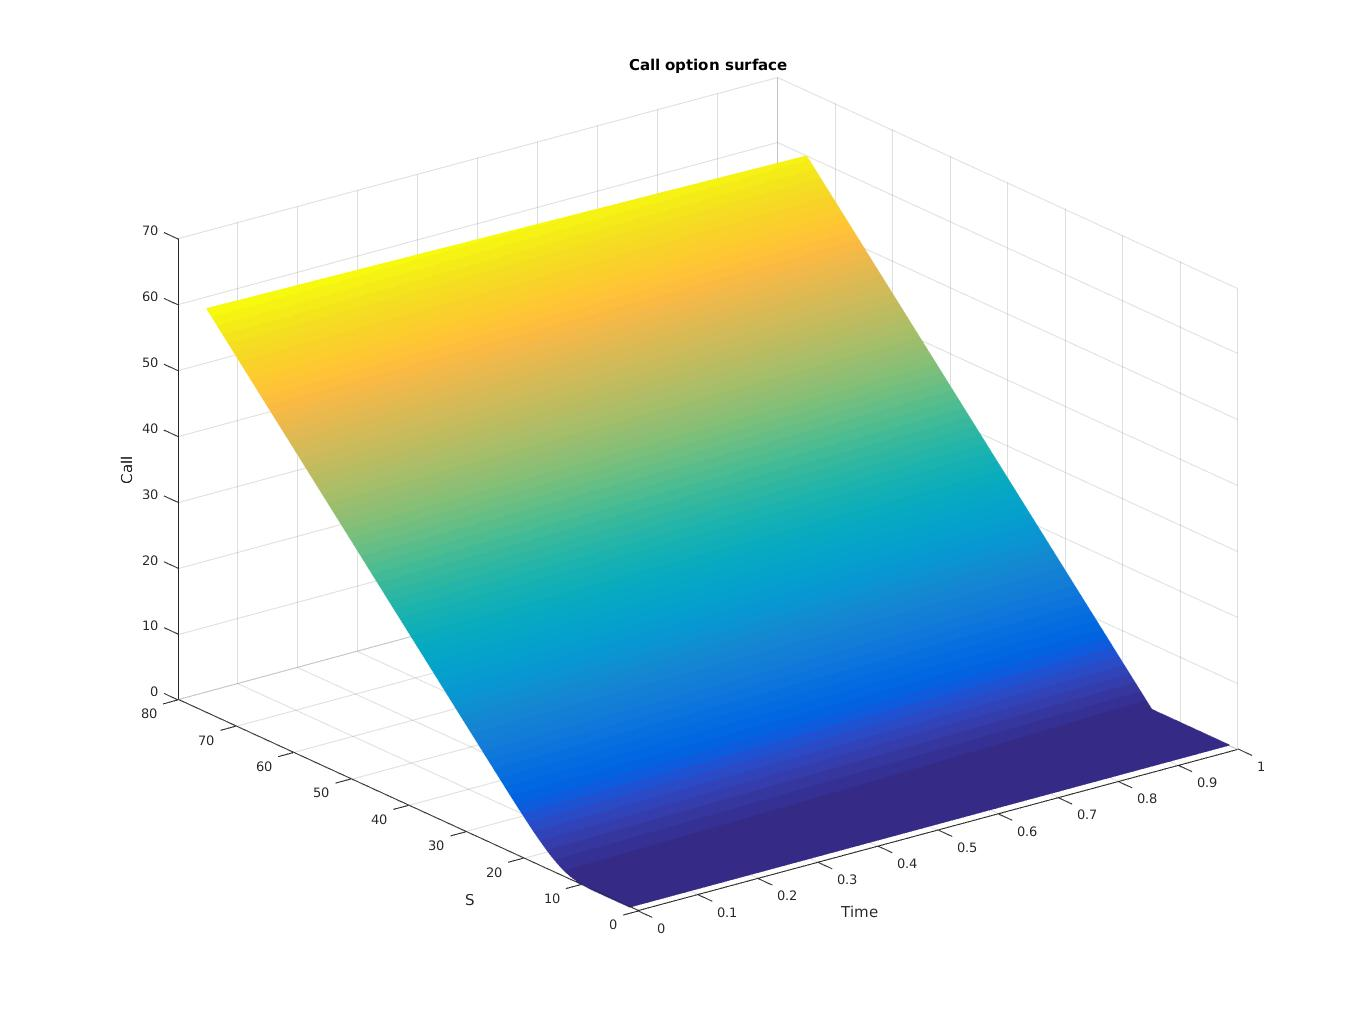
\includegraphics[width=0.8\linewidth]{BS_surface.jpg}
   \caption{Call option surface obtained by solving the Black-Scholes PDE. It is computed with the parameters in Table \ref{tab:BS}}
   \label{BS_surface} 
\end{figure}

The \cite{BS73} model assumes a geometric Brownian motion for the dynamics of the underlying, as we saw in (\ref{GBM2}).
It corresponds to the exponential of a Lévy process $\{X_t\}_{t\geq 0}$ with triplet $(b,\sigma,0)$, with Lévy measure $\nu = 0$.
The BS PDE (\ref{PIDE_log}) in log-variables turns out to be
\begin{equation}\label{BS_PDE}
\frac{\partial  V(t,x)}{\partial t}  
          + \biggl( r -\frac{1}{2}\sigma^2 \biggr) \frac{\partial V(t,x)}{\partial x}
          + \frac{1}{2} \sigma^2 \frac{\partial^2  V(t,x)}{\partial x^2} - r  V(t,x)  = 0.
\end{equation}
The Lévy measure is identically null and therefore there is no integral term.
The domain is restricted to $[t_0,T]\, \times \, [A_1,A_2]$. We apply the IMEX scheme, that in this case is a fully implicit scheme.  
The discretized equation becomes
\begin{align}
&\frac{V^{n+1}_{i} -V^{n}_{i}}{\Delta t} + 
(r-\frac{1}{2}\sigma^2) \frac{V^{n}_{i+1} -V^{n}_{i-1}}{ 2 \Delta x} \\ \nonumber
&+ \frac{1}{2} \sigma^2 \frac{V^{n}_{i+1} + V^{n}_{i-1} - 2 V^{n}_{i}}{\Delta x^2}  - r V^{n}_i = 0.
\end{align}
Rearranging the terms: 
\begin{align*}
 V^{n+1}_{i} &= V^{n}_{i} \biggl( 1 + r\Delta t + \sigma^2 \frac{\Delta t}{h_x^2} \biggr)  \\
& + V^{n}_{i+1} \biggl( -(r -\frac{1}{2}\sigma^2)\frac{\Delta t}{2 \Delta x} +
\frac{1}{2}\sigma^2 \frac{\Delta t}{\Delta x^2}  \biggr)  \\
& + V^{n}_{i-1} \biggl( (r -\frac{1}{2}\sigma^2)\frac{\Delta t}{2 \Delta x} + 
\frac{1}{2}\sigma^2 \frac{\Delta t}{\Delta x^2}  \biggr).
\end{align*}
We can rename the coefficients such that:
$$ V^{n+1}_{i} = a V^{n}_{i-1} + b V^{n}_{i} + c V^{n}_{i+1}, $$
and write it in matrix form:
\begin{figure}[t]
   \centering
   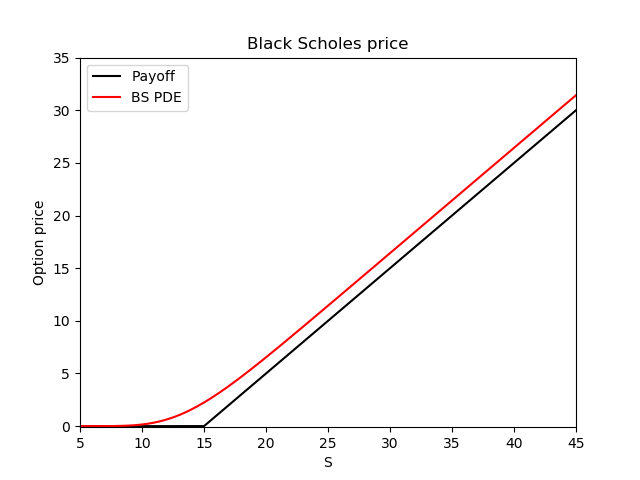
\includegraphics[width=0.7\linewidth]{BS_call.png}
   \caption{Price of a call option at time $t=0$ with parameters in Table \ref{tab:BS}.}
   \label{BS_call}
\end{figure}  
$$
\left(
\begin{array}{c}
V^{n+1}_{1} \\
V^{n+1}_{2} \\
\vdots \\
V^{n+1}_{M-2} \\
V^{n+1}_{M-1} \\
\end{array}
\right) = 
\underbrace{
\left(
\begin{array}{ccccc}
b     & c  & 0 & \cdots  & 0 \\
a     & b  & c & 0  & 0  \\
0      & \ddots & \ddots &   \ddots     & 0  \\
\vdots & 0 & a & b  & c  \\
0      & 0 & 0 & a  & b \\
\end{array}
\right) }_{\mathcal{D}} \cdot
\left(
\begin{array}{c}
V^{n}_{1} \\
V^{n}_{2} \\
\vdots \\
V^{n}_{M-2} \\
V^{n}_{M-1} 
\end{array}
\right)
+ \underbrace{
\left(
\begin{array}{c}
 a V^{n}_{0} \\
  0 \\
 \vdots \\
 0 \\
c V^{n}_{M} \\
\end{array}
\right) }_{\mbox{B (boundary terms)}}
$$
The system 
$$ V^{n+1}_{i} = \mathcal{D} V^{n}_{i} + B \quad \mbox{ for } \quad 1 \leq i \leq M-1$$
can be solved easily for $V^{n}_{i}$ by inverting\footnote{ 
Matrix inversion is a slow operation and there are plenty of efficient algorithms that permit to solve a linear system with no need of matrix inversion.
In this thesis we solved all the linear systems occurring after the implicit discretization of a PDE (or PIDE) with the LU decomposition method.}
the matrix $\mathcal{D}$.
\begin{table}[!h]
\centering
{\begin{tabular}{llll}
\toprule
 \multicolumn{4}{c}{BS Parameters} \\
\midrule
$K$ & $T$ & $r$ & $\sigma$ \\
15 & 1 & 0.1 & 0.25 \\
\bottomrule
\end{tabular}}
\caption{Option parameters and diffusion process parameters.}
\label{tab:BS}		
\end{table}

Using the parameters in Table \ref{tab:BS} we can solve the linear system and plot the solution in Figures \ref{BS_surface} and \ref{BS_call}.



\subsection{Merton PIDE}


We presented the Merton model in Section \ref{Merton_section}. 
Let us recall that the jump component of the Merton process has finite activity, $\nu(\R) = \lambda < \infty$.
Following Eq. (\ref{PIDE_log}), the Merton PIDE in log-variables has the following form: 
\begin{align}\label{Merton_PIDE}
&  \frac{\partial V(t,x)}{\partial t} - r V(t,x) 
          + \biggl( r -\frac{1}{2}\sigma^2 -m \biggr) \frac{\partial V(t,x)}{\partial x} \\ \nonumber
          &+ \frac{1}{2} \sigma^2 \frac{\partial^2 V(t,x)}{\partial x^2} 
          + \int_{\R} V(t,x+z) \nu(dz) - \lambda V(t,x)  = 0.
\end{align}
with $m$ defined in (\ref{parameter_m}).
Since we have to restrict the problem to a bounded region, we consider the equation (\ref{restricted_domain}):
\begin{align*}
&  \frac{\partial V(t,x)}{\partial t} - r V(t,x) 
          + \biggl( r -\frac{1}{2}\sigma^2 - \hat m \biggr) \frac{\partial V(t,x)}{\partial x} \\
          &+ \frac{1}{2} \sigma^2 \frac{\partial^2 V(t,x)}{\partial x^2} 
          + \int_{-B_1}^{B_2} V(t,x+z) \nu(dz) - \hat \lambda V(t,x)  = 0.
\end{align*}
with $\hat m = \int_{-B_1}^{B_2} \bigl( e^z-1 \bigr) \nu(dz)$ and $\hat \lambda = \int_{-B_1}^{B_2} \nu(dz)$.

For $0 < K_1 < K_2$ we choose $B_1,B_2$ such that $ \bigl[-B_1,B_2\bigr] = \bigl[ ( -K_1-1/2 )\Delta x , ( K_2+1/2 )\Delta x \bigr] $.
Let us discretize the integral as follows:
\begin{equation}\label{trap_quad}
 \int_{-B_1}^{B_2}  V(t_n,x_i+z) \nu(dz) \approx \sum_{k = -K_1}^{K_2} \nu_k V^{n}_{i+k}
\end{equation}
where
\begin{equation}\label{nu1}
 \nu_k = \int_{(k-\frac{1}{2}) \Delta x}^{(k+\frac{1}{2}) \Delta x} \nu(z) dz, \hspace{1em} \mbox{ for } \hspace{1em} -K_1 \leq k \leq K_2. 
\end{equation}
We have that $ \hat \lambda = \sum_{k = -K_1}^{K_2} \nu_k $. For large values of $B_1$ and $B_2$, the parameter $\hat \lambda$ is a good approximation for $\lambda$, since
$$\lambda = \lim_{B_1,B_2 \to \infty} \hat \lambda = \lim_{B_1,B_2 \to \infty} \int_{-B_1}^{B_2} \nu(dz).$$
The discretized equation using the IMEX scheme becomes: 
\begin{align}
&\frac{V^{n+1}_{i} -V^{n}_{i}}{\Delta t} + 
(r-\frac{1}{2}\sigma^2 - \hat m) \frac{V^{n}_{i+1} -V^{n}_{i-1}}{ 2 \Delta x} \\ \nonumber
&+ \frac{1}{2} \sigma^2 \frac{V^{n}_{i+1} + V^{n}_{i-1} - 2 V^{n}_{i}}{\Delta x^2}  - (r+\hat \lambda) V^{n}_i +\sum_{k = -K_1}^{K_2} \nu_k V^{n+1}_{i+k} = 0.
\end{align}
Rearranging the terms: 
\begin{align*}
\underbrace{ V^{n+1}_{i} + \Delta t \sum_{k = -K_1}^{K_2} \nu_k V^{n+1}_{i+k} }_{\tilde V^{n+1}_i} &= 
	V^{n}_{i} \biggl( 1 + (r+\hat \lambda)\Delta t + \sigma^2 \frac{\Delta t}{\Delta x^2} \biggr)  \\
& + V^{n}_{i+1} \biggl( -(r -\frac{1}{2}\sigma^2 -\hat m )\frac{\Delta t}{2 \Delta x} +
\frac{1}{2}\sigma^2 \frac{\Delta t}{\Delta x^2}  \biggr)  \\
& + V^{n}_{i-1} \biggl( (r -\frac{1}{2}\sigma^2 - \hat m)\frac{\Delta t}{2 \Delta x} + 
\frac{1}{2}\sigma^2 \frac{\Delta t}{\Delta x^2}  \biggr).
\end{align*}
We can rename the coefficients:
$$ \tilde V^{n+1}_{i} = a V^{n}_{i-1} + b V^{n}_{i} + c V^{n}_{i+1}, $$
and solve the system for $V^{n}_{i}$:
\begin{equation*}
 \begin{cases}
  \tilde V^{n+1}_i = V^{n+1}_{i} + \Delta t \sum_{k = -K_1}^{K_2} V^{n+1}_{i+k} \nu_k \\
  V^{n}_{i} = \mathcal{D}^{-1} \biggl( \tilde V^{n+1}_{i} - B \biggr) \quad \mbox{ for } \quad 1 \leq i \leq M-1  
 \end{cases}
\end{equation*}
where $\mathcal{D}$ is the tridiagonal matrix formed by the coefficients $a,b,c$, and with boundary terms $B = (a V^{n}_{0}, 0, ... , 0, c V^{n}_{M})$.  
\begin{figure}[t]
   \centering
   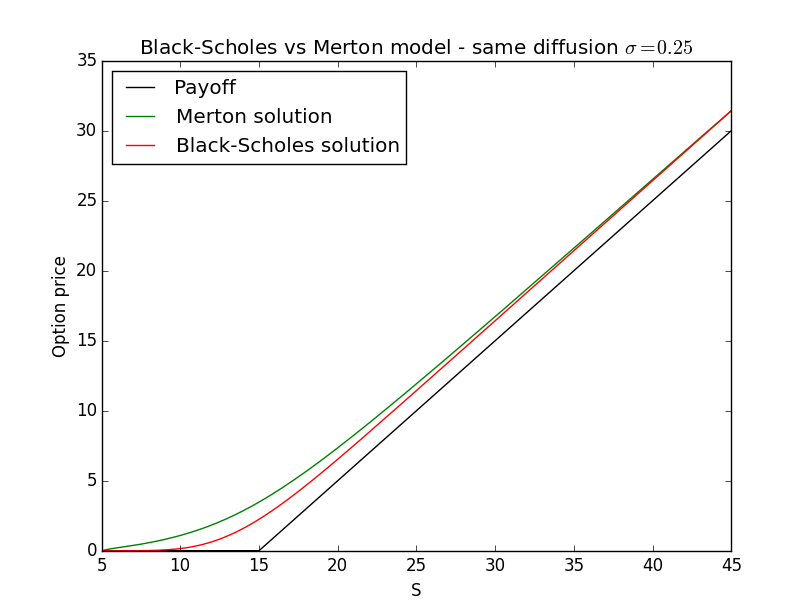
\includegraphics[width=0.7\linewidth]{BS_Merton.png}
   \caption{Comparison of prices of a call option at time $t=0$ for BS and Merton models. The parameters are in Tables \ref{tab:BS} and \ref{tab:Mert} (first line).}
   \label{BS_Merton}
\end{figure}  
\begin{figure}[t]
   \centering
   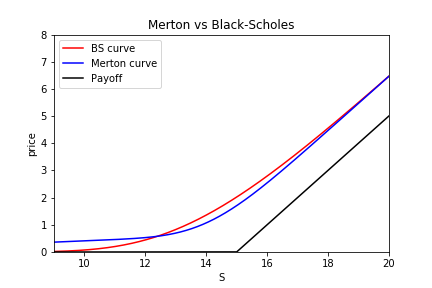
\includegraphics[width=0.7\linewidth]{Mert-BS_same_var.png}
   \caption{Comparison of prices of a call option at time $t=0$ for Merton and BS models with same standard deviation. The Merton parameters are those in the second line of
   the Table \ref{tab:Mert}, while the diffusion parameter $\sigma$ for the BS prices is chosen such that the variances of the two processes are the same. }
   \label{BS_Merton2} 
 \end{figure}

\begin{table}[t]
  \centering
  \begin{tabular}{cccccccc}
  \toprule
  \multicolumn{8}{c}{Merton parameters} \\
  \midrule
  Figure & $K$ & $T$ & $r$ & $\sigma$ & $\alpha$ &$\xi$ & $\lambda$ \\
  \midrule
  Fig. \ref{BS_Merton} & 15 & 1 & 0.1 & 0.25 & 0 & 0.5 & 0.8 \\
  Fig. \ref{BS_Merton2} & 15 & 1 & 0.1 & 0.1 & 0 & 1.8 & 0.01 \\
  \bottomrule
  \end{tabular}
  \caption{Option's parameters and Merton process parameters.}
  \label{tab:Mert}
\end{table}
In Figure \ref{BS_Merton} we computed the BS and Merton curves using the parameters in Tables \ref{tab:BS} and \ref{tab:Mert}. 
The Merton curve is everywhere higher than the BS curve. 
This is a consequence 
of the additional jump component in the Merton process that increases the total variance. 
The two processes have same diffusion component $\sigma$, 
but the Merton process has total variance $\sigma^2 + \lambda \xi^2 +\lambda \alpha^2$, while the diffusion process has only variance $\sigma^2$.

In order to investigate the effect of the heavy tails on the shape of the option curve, let us consider the second set of parameters in Table \ref{tab:Mert}. 
Under these parameters, the Merton distribution has a very high kurtosis ($\kappa = 97.32$). 
In Figure \ref{BS_Merton2} we compare the Merton curve with a BS curve computed using the volatility parameter 
$\sigma_{BS} = \sqrt{\sigma^2 + \lambda \xi^2 +\lambda \alpha^2 }$. 
In this way, the differences in the shape are only due to the kurtosis, since both processes have zero skewness and equal mean and variance. 

As expected, the BS curve is smaller than the Merton curve in the \emph{deep out of the money} region (in the picture \ref{BS_Merton2} this region corresponds to $S<12$). 
This is a consequence of the heavy tails distribution of the Merton process, that assigns more probability to large movements of the underlying, i.e. a deep out of the money
option has more probability to return \emph{in the money} (where $S>K$).


\subsection{Variance Gamma PIDE}\label{VG_section2}

We introduced the Variance Gamma process in Section \ref{VG_section}. The VG process has infinite activity i.e.
$\nu(\R) = \infty$ and has the triplet presented in (\ref{VG_triplet}). 
 
From the general PIDE pricing formula (\ref{PIDE_log}), we obtain the VG PIDE for a function $V \in C^{1,1}([0,T] \times \R) \bigcap \mathcal{C}_2([0,T] \times \R)$:
\begin{equation} \label{VG_PIDE}
 \frac{\partial V(t,x)}{\partial t} + (r-w) \frac{\partial V(t,x)}{\partial x}
 + \int_{\R} \bigl[ V(t,x+z) - V(t,x) \bigr] \nu(dz) = rV(t,x) .
\end{equation}
with $w$ defined in (\ref{parameter_w}).

Unfortunately, it is not possible to apply the IMEX discretization directly to this equation. The Lévy measure has a singularity in the origin,
that should be removed before the discretization.

An idea to overcome this problem, that can be applied to any Lévy processes with infinite activity, is presented in \cite{CoVo05b}. 
The authors propose to approximate the process $\{X_t\}_{t\geq0}$ by an
appropriate finite activity process with a modified diffusion component.
The ``small jumps'' martingale component is approximated by a Brownian motion with same variance.
After fixing a truncation parameter $\epsilon >0$, the integrals in the SDE are split in two domains: $\{|z|<\epsilon\}$ and $\{|z|\geq \epsilon\}$.
The integrand on the domain $\{ |z|<\epsilon \}$, is approximated by the Taylor expansion 
 $e^z-1-z = \frac{z^2}{2} + \mathcal{O}(z^3)$ such that
\begin{align}\label{log_sde_inf_act}\nonumber
  dX_t =& \biggl( \mu-\frac{1}{2}\sigma^2 - \int_{\R} \bigl( e^z-1-z \bigr) \nu(dz) \biggr)dt + \sigma dW + + \int_{\R} z \tilde N(dt,dz) \\ \nonumber
       =& \biggl( \mu - \frac{1}{2}\sigma^2 -\int_{|z|<\epsilon} (e^z-1-z) \nu(dz) -\int_{|z|\geq \epsilon} (e^z-1-z) \nu(dz)  \biggr) dt\\ \nonumber
        &+ \sigma dW_t + \underbrace{\int_{|z|< \epsilon} z \tilde N(dt,dz)}_{\sigma_{\epsilon} dW_t} + \int_{|z| \geq \epsilon} z \tilde N(dt,dz) \\ 
       =& \biggl( \mu - \frac{1}{2} (\sigma^2 + \sigma_{\epsilon}^2) - w_{\epsilon} + \lambda_{\epsilon} \theta_{\epsilon}  \biggr) dt + \bigl( \sigma+\sigma_{\epsilon}\bigr) dW_t 
       + \int_{|z|\geq \epsilon} z \tilde N(dt,dz) ,
\end{align}
where we defined the new parameters
\begin{align}\label{sig_eps}
 & \sigma_{\epsilon}^2 :=  \int_{|z| < \epsilon} z^2 \nu(dz), \quad \quad w_{\epsilon} := \int_{|z| \geq \epsilon} (e^z-1) \nu(dz), \\ \nonumber
 & \lambda_{\epsilon} :=  \int_{|z| \geq \epsilon} \nu(dz), \quad \quad \theta_{\epsilon} := \frac{1}{\lambda_{\epsilon}} \int_{|z| \geq \epsilon} z \nu(dz) .
\end{align}
The process $\int_{|z|\geq \epsilon} z \tilde N(dt,dz)$ is a compensated Poisson process with finite activity $\lambda_{\epsilon}$ 
and variance $\sigma_J^2 = \int_{|z| \geq \epsilon} z^2 \nu(dz) $.

For the VG process, where $\sigma = 0$ the approximated dynamics is thus
\begin{equation}\label{log_sde_VG}
dX_t = \biggl( \mu - \frac{1}{2} \sigma_{\epsilon}^2 - w_{\epsilon} + \lambda_{\epsilon} \theta_{\epsilon}  \biggr) dt 
       + \sigma_{\epsilon} dW_t + \int_{|z|\geq \epsilon} z \tilde N(dt,dz),
\end{equation}
where the parameters are obtained from the Lévy measure (\ref{VG_measure}).

For any $V\in C^2(\R) \bigcap C_2(\R)$, the infinitesimal generator associated with (\ref{log_sde_VG}) has a ``jump-diffusion'' form
\begin{align}\label{VG_inf_gen}
\LL^{VG} V(x) \; =& \; \bigl( \mu-\frac{1}{2}\sigma_{\epsilon}^2 - w_{\epsilon} \bigr) \frac{\partial V}{\partial x} 
+ \frac{1}{2}\sigma_{\epsilon}^2 \frac{\partial^2 V}{\partial x^2} \\ \nonumber
&+ \int_{|z| \geq \epsilon} V(x+z) \nu(dz) - \lambda_{\epsilon} V(x).
\end{align}
The same result can be obtained directly from the infinitesimal generator (\ref{RN_log_gen}) with $\sigma =0$:
\begin{align*}
\LL^{VG} V(x) =& \; \mu \frac{\partial V}{\partial x}
+ \int_{|z| < \epsilon}
\biggl[ V(x+z) - V(x) - (e^z-1)\frac{\partial V}{\partial x} \biggr] \nu(dz) \\
&+ \int_{|z| \geq \epsilon}
\biggl[ V(x+z) - V(x) - (e^z-1)\frac{\partial V}{\partial x} \biggr] \nu(dz),
\end{align*}
In the integral term on the domain $\{ |z|<\epsilon \}$, we have to assume a smooth enough $V$ such that we can use the following Taylor approximation
\begin{itemize}
 \item $V(x+z) = V(x) + \frac{\partial V}{\partial x} z + \frac{1}{2} \frac{\partial^2 V}{\partial x^2} z^2 + \mathcal{O}(z^3)$.
 \item $e^z-1 = z + \frac{z^2}{2} + \mathcal{O}(z^3) $.
\end{itemize}
Considering only the terms up to the second order, the integral for $\{ |z| < \epsilon \}$ is
\begin{equation*}
 \int_{|z| < \epsilon} \frac{z^2}{2}
\biggl[ \frac{\partial^2 V}{\partial x^2} - \frac{\partial V}{\partial x} \biggr] \nu(dz)
= \frac{\sigma_{\epsilon}^2}{2} \biggl[ \frac{\partial^2 V}{\partial x^2} - \frac{\partial V}{\partial x} \biggr],
\end{equation*}
and we get again the infinitesimal generator (\ref{VG_inf_gen}).
Using this generator and equations (\ref{derivative_PIDE}) and (\ref{mu=r}), the final PIDE is thus
\begin{align}\label{VG_JD}
&  \frac{\partial V(t,x)}{\partial t} +
 \bigl( r-\frac{1}{2}\sigma_{\epsilon}^2 - w_{\epsilon} \bigr) \frac{\partial V(t,x)}{\partial x} 
 + \frac{1}{2}\sigma_{\epsilon}^2 \frac{\partial^2 V(t,x)}{\partial x^2} \\ \nonumber
 &+ \int_{|z| \geq \epsilon} V(t,x+z) \nu(dz) = (\lambda_{\epsilon} + r) V(t,x).
\end{align}

\begin{figure}[!t]
   \centering
   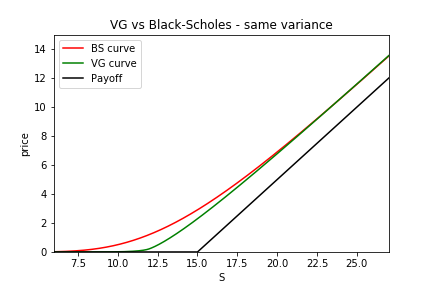
\includegraphics[width=0.7\linewidth]{VG-BS_theta_negative.png}
   \caption{\textbf{Negative skewness:} Comparison of call option curves at $t=0$ for VG and BS models. The VG parameters are in Table (\ref{tab:VG}). The BS curve is computed with a 
   $\sigma_{BS} = \sqrt{\bar\sigma^2 + \theta^2 \kappa}$, such that the two processes have same variance.}
   \label{BS_VG} 
 \end{figure}
\begin{table}[h]
  \centering
  \begin{tabular}{ccccccc}
  \toprule
  \multicolumn{7}{c}{VG parameters} \\
  \midrule
  Figure & $K$ & $T$ & $r$ & $\theta$ & $\bar\sigma$ &$\kappa$ \\
  \midrule
  Fig. \ref{BS_VG} & 15 & 1 & 0.1 & -0.2 & 0.2 & 2.5 \\
  Fig. \ref{BS_VG2} & 15 & 1 & 0.1 & 0.2 & 0.2 & 2.5 \\
  \bottomrule
  \end{tabular}
  \caption{Option's parameters and VG process parameters.}
  \label{tab:VG}
\end{table}

This equation is almost identical to equation (\ref{Merton_PIDE}), except for the truncation in the integral. 
At this point we can restrict the computational domain on $[A_1,A_2]$ and the integral region on $[-B_1,B_2]$ and using the same discretization
used for the Merton PIDE, we can solve the problem with the IMEX scheme.\\

Using the parameters in Table \ref{tab:VG} we compute VG call option prices and compare them with BS prices with volatility $\sigma_{BS} = \sqrt{\bar\sigma^2 + \theta^2 \kappa}$, 
such that the two processes have same variance.
In this way, only the features coming from skewness and kurtosis should pop up.
Under this choice of parameters the VG process has standard deviation equal to $0.37$, skewness (in absolute value) $3.05$ and kurtosis $14.38$.
The sign of the skewness is determined by the sign of the parameter $\theta$.

In Figures \ref{BS_VG} and \ref{BS_VG2} we compare the BS and VG curves.
This example wants to show how different the shape of the VG curves can be by modifying the skewness parameter.

The reader can consult \cite{Schoutens} for further information on Merton and VG processes and on general numerical tests and calibration of exponential Lévy processes. 
\begin{figure}[!t]
   \centering
   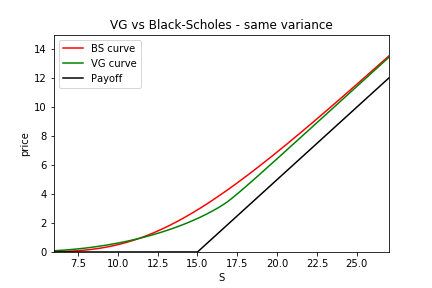
\includegraphics[width=0.7\linewidth]{VG-BS_theta_positive.png}
   \caption{\textbf{Positive skewness:} Comparison of call option curves at $t=0$ for VG and BS models. The VG parameters are in Table \ref{tab:VG}. The BS curve is computed with a 
   $\sigma_{BS} = \sqrt{\bar\sigma^2 + \theta^2 \kappa}$, such that the two processes have same variance.}
   \label{BS_VG2} 
\end{figure}



\subsection{Numerical convergence analysis}\label{numerical_concergence_section}

\begin{table}[ht]
\centering
\begin{tabular}[t]{ccc}
\toprule
       &  \textbf{Closed formula} &  \textbf{PDE/PIDE} \\
\midrule
BS      &  2.246368  & 2.246352 \\
Merton  &  3.477645  & 3.477468 \\ 
VG      &  1.987006  & 1.987089 \\
\bottomrule
\end{tabular}
\caption{Option prices with $S_0=K=15$ and $T=1$. Black Scholes parameters are in Table \ref{tab:BS}. Merton parameters are in the first line of Table \ref{tab:Mert}.
The Variance Gamma parameters are $\theta=-0.1$, $\bar \sigma = 0.2$, $\kappa = 0.1$.}
\label{tab:prices_BS_M_VG}
\end{table}%

In Table \ref{tab:prices_BS_M_VG} we compare the ATM (\emph{at the money}) prices of a European call option computed with the algorithms presented 
in the previous sections, with the prices obtained by closed formulas.
For the BS model, we used the well known closed formula presented in the paper \cite{BS73}. 
In order to compute the Merton price we use the semi-closed formula derived in \cite{Me76},
and for the VG price we used the semi-closed formula of \cite{MCC98}. 
The PIDE prices are obtained by solving the equations (\ref{BS_PDE}), (\ref{Merton_PIDE}) and (\ref{VG_JD}).
In this analysis we consider the same sets of parameters that we will use in Chapter \ref{Chapter6} (see Table \ref{tab:ATM_price}).

It is a common practice to select the upper-bound and lower-bound of the price as a multiple of the strike price. 
In our case we set $S_{max} = 6K$ and $S_{min} = K/6$.
According to this choice, we set $A_1 = \log(K/6)$ and $A_2 = \log(6K)$ for all the three considered problems.
 
For the Merton PIDE we set $B_1 = B_2 = 5\sigma_M$, with $\sigma_M = \sqrt{ \lambda \xi^2 + \lambda \alpha^2 }$. 
For the VG PIDE we set $ B_1 = B_2 = 5 \sigma_{VG}$, with $\sigma_{VG} = \sqrt{\bar\sigma^2 + \theta^2 \kappa}$. 
In both cases, the parameters $B_1$ and $B_2$ are multiple of the standard deviation of the respective jump processes.
The parameters $A_1$, $A_2$, $B_1$ and $B_2$ are very important and should be set as large as possible in order to have an accurate result.
\begin{table}[ht]
\centering
\begin{tabular}[t]{cccc}
\toprule
   \textbf{space steps}    &  \textbf{BS} &  \textbf{Merton}  & \textbf{VG} \\
\midrule
 50    & 2.268400  &  3.495694  &  2.032549  \\
 100   & 2.251734  &  3.481931  &  2.014171  \\
 200   & 2.247682  &  3.478573  &  2.004308  \\
 400   & 2.246682  &  3.477744  &  1.998356 \\ 
 800   & 2.246433  &  3.477537  &  1.994912 \\
 1600  & 2.246371  &  3.477486  &  1.992661 \\
 3200  & 2.246356  &  3.477473  &  1.990863 \\
 6400  & 2.246352  &  3.477469  &  1.989213 \\
% 12800 & 2.246351  &  3.477469  &  1.987604 \\
\bottomrule
\end{tabular}
\caption{Convergence table. Fixed 12000 time steps. }
\label{tab:space_conv}
\end{table}%
\begin{table}[ht]
\centering
\begin{tabular}[t]{cccc}
\toprule
   \textbf{time steps}    &  \textbf{BS} &  \textbf{Merton}  & \textbf{VG} \\
\midrule
50     & 2.242021 & 3.440676 & 0.998308 \\
100    & 2.244216 & 3.459215 & 1.295962 \\
200    & 2.245297 & 3.468434 & 1.554740 \\
400    & 2.245834 & 3.473032 & 1.741888 \\
800    & 2.246102 & 3.475328 & 1.858731 \\
1600   & 2.246235 & 3.476475 & 1.924853 \\
3200   & 2.246302 & 3.477048 & 1.960160 \\
6400   & 2.246335 & 3.477335 & 1.978422 \\
%10000  & 2.246347 & 3.477438 & 1.985100 \\
\bottomrule
\end{tabular}
\caption{Convergence table. Fixed 16000 space steps. }
\label{tab:time_conv}
\end{table}%

The PDE/PIDE prices in Table \ref{tab:prices_BS_M_VG} are obtained by dividing the space interval $[A_1,A_2]$ in $M=16000$ steps and the time interval $[t_0,T]$ in $N=12000$ steps.
%\footnote{In the Merton and VG problems, the intervals $[-B_1,A_1]$ and $[A_2,B_2]$ contain additional 11161 and 4520 space steps respectively.}
We can see that BS and VG prices are accurate up to the fourth decimal digit and Merton is accurate up to the third decimal digit. 
In the following analysis we assume they are the correct limiting 
value of the numerical algorithm, and indicate them by $V^* = \lim_{M,N \to \infty} V^{M,N}$.

In Tables \ref{tab:space_conv} we computed option prices $V^M$, by varying the number of space steps $M$ and keeping the time steps fixed $N=12000$.
In Table \ref{tab:time_conv} we did the opposite i.e. we computed $V^N$ for different values of $N$ and constant $M=16000$.
From these values it is possible to investigate how the error changes with respect to the discretization step.

Let us consider for instance the space discretization. 
If we define the error $\varepsilon_M = |V^M - V^*|$, we can assume that it has a polynomial relation with the discretization step $\Delta x = \frac{A_2 - A_1}{M}$ i.e. 
$\varepsilon_M \propto (\frac{1}{M})^p$, where $p$ is the \textbf{order of convergence}.
In the Table \ref{tab:space_conv} we chose $M$ in a smart way such that $M = 50\cdot2^n$, for $0 \leq n \leq 7$. We can take the $\log_2$ on both sides such that
\begin{equation}
 - \log_2 \varepsilon_n = C + np,
\end{equation}
where $C\in \R$ is a constant of proportionality. 
The same analysis can be done for the time discretization.
\begin{figure}[t!]
 \begin{minipage}[b]{0.5\linewidth}
   \centering
 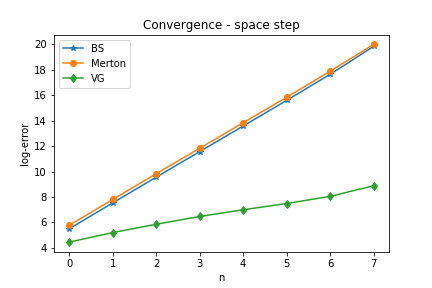
\includegraphics[width=\linewidth]{space_convergence.png}
 % EU_call.png: 0x0 pixel, 300dpi, 0.00x0.00 cm, bb=
 \caption{Log-error of the prices in Table \ref{tab:space_conv}.}
 \label{fig_space}
  \end{minipage}
 \ \hspace{2mm} \hspace{3mm} \
 \begin{minipage}[b]{0.5\linewidth}
 \centering
 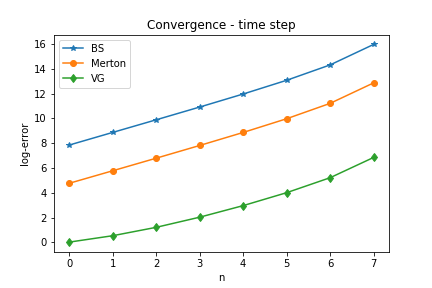
\includegraphics[width=\linewidth]{time_convergence.png}
 % EU_call.png: 0x0 pixel, 300dpi, 0.00x0.00 cm, bb=
 \caption{Log-error of the prices in Table \ref{tab:time_conv}.}
 \label{fig_time}
 \end{minipage}
\end{figure}

The theoretical order of convergence of the implicit scheme applied to the BS PDE is $p=2$ for the space discretization and $p=1$ for the time discretization.
For a discussion on the convergence rate for IMEX schemes applied to PIDEs we refer to \cite{CoVo05b} (Section 6.4). 
Since the theoretical analysis of convergence for IMEX schemes is a wide topic, in this thesis we just perform a numerical convergence analysis.

In the two pictures \ref{fig_space} and \ref{fig_time} we plotted the log-error $- \log_2 \varepsilon_n$ for the values 
in the Tables \ref{tab:space_conv} and \ref{tab:time_conv} respectively.
It turns out that both the BS and Merton prices have a quadratic error ($p=2$) in space, while VG prices have a convergence order much smaller ($p\sim 0.8$). 
It is worth to mention that in our algorithm we choose the truncation parameter $\epsilon = 1.5 \Delta x$.
This choice not only influences the convergence of the numerical scheme, but also the convergence of the Brownian approximation, since the parameters in (\ref{sig_eps}) depend on 
$\epsilon$.\\
According to the results of Figure \ref{fig_time}, the time error is linear ($p=1$) for all the three models.



\section{Chapter conclusions}


This chapter exposes in brief  
the main concepts of the ``No-arbitrage'', or ``martingale'', pricing theory. 

This is the most common approach used to price financial derivatives. 
The well known Black-Scholes model is included in this framework as a special case when the stock dynamics follows
a geometric Brownian motion. 
The martingale pricing theory applies to all exponential Lévy processes that satisfy the assumption \textbf{EM}.
For the purpose of this thesis, the contents of this chapter are quite important because we will use them to make comparisons 
with the more complex models introduced in the next chapters.

In Section \ref{No_arbitrage_theory} we present the fundamental concepts necessary to define the pricing function of a derivative contract.
Then we prove that this pricing function is the solution of a partial integro-differential equation when the stock dynamics follows an exponential Lévy process.

In the second part of the chapter, Section \ref{Finite_difference_methods}, we describe the algorithm used for the numerical solution of the Black-Scholes PDE and the
Merton and VG PIDEs.
We explain how to discretize the PIDE using the IMEX finite difference method proposed in \cite{CoVo05b}. We also provide a numerical convergence analysis of this method.
The numerical results of this chapter will be used for comparison in Chapters \ref{Chapter3} and \ref{Chapter6}.
In Chapter \ref{Chapter3} we compare the prices obtained by the multinomial method with those obtained by solving the VG PIDE.  
In Chapter \ref{Chapter6}, instead, we will see that when the transaction costs go to zero, 
the prices obtained from the transaction costs model are equal to the prices obtained by the martingale pricing theory.

%The python code for the algorithms presented in this chapter can be found in the github page \url{https://github.com/cantaro86}. 
